\documentclass[]{article}
\usepackage{lmodern}
\usepackage{amssymb,amsmath}
\usepackage{ifxetex,ifluatex}
\usepackage{fixltx2e} % provides \textsubscript
\ifnum 0\ifxetex 1\fi\ifluatex 1\fi=0 % if pdftex
  \usepackage[T1]{fontenc}
  \usepackage[utf8]{inputenc}
\else % if luatex or xelatex
  \ifxetex
    \usepackage{mathspec}
  \else
    \usepackage{fontspec}
  \fi
  \defaultfontfeatures{Ligatures=TeX,Scale=MatchLowercase}
\fi
% use upquote if available, for straight quotes in verbatim environments
\IfFileExists{upquote.sty}{\usepackage{upquote}}{}
% use microtype if available
\IfFileExists{microtype.sty}{%
\usepackage{microtype}
\UseMicrotypeSet[protrusion]{basicmath} % disable protrusion for tt fonts
}{}
\usepackage[margin=1in]{geometry}
\usepackage{hyperref}
\hypersetup{unicode=true,
            pdftitle={numpy in python},
            pdfauthor={Matrix\_Chen},
            pdfborder={0 0 0},
            breaklinks=true}
\urlstyle{same}  % don't use monospace font for urls
\usepackage{color}
\usepackage{fancyvrb}
\newcommand{\VerbBar}{|}
\newcommand{\VERB}{\Verb[commandchars=\\\{\}]}
\DefineVerbatimEnvironment{Highlighting}{Verbatim}{commandchars=\\\{\}}
% Add ',fontsize=\small' for more characters per line
\usepackage{framed}
\definecolor{shadecolor}{RGB}{248,248,248}
\newenvironment{Shaded}{\begin{snugshade}}{\end{snugshade}}
\newcommand{\KeywordTok}[1]{\textcolor[rgb]{0.13,0.29,0.53}{\textbf{#1}}}
\newcommand{\DataTypeTok}[1]{\textcolor[rgb]{0.13,0.29,0.53}{#1}}
\newcommand{\DecValTok}[1]{\textcolor[rgb]{0.00,0.00,0.81}{#1}}
\newcommand{\BaseNTok}[1]{\textcolor[rgb]{0.00,0.00,0.81}{#1}}
\newcommand{\FloatTok}[1]{\textcolor[rgb]{0.00,0.00,0.81}{#1}}
\newcommand{\ConstantTok}[1]{\textcolor[rgb]{0.00,0.00,0.00}{#1}}
\newcommand{\CharTok}[1]{\textcolor[rgb]{0.31,0.60,0.02}{#1}}
\newcommand{\SpecialCharTok}[1]{\textcolor[rgb]{0.00,0.00,0.00}{#1}}
\newcommand{\StringTok}[1]{\textcolor[rgb]{0.31,0.60,0.02}{#1}}
\newcommand{\VerbatimStringTok}[1]{\textcolor[rgb]{0.31,0.60,0.02}{#1}}
\newcommand{\SpecialStringTok}[1]{\textcolor[rgb]{0.31,0.60,0.02}{#1}}
\newcommand{\ImportTok}[1]{#1}
\newcommand{\CommentTok}[1]{\textcolor[rgb]{0.56,0.35,0.01}{\textit{#1}}}
\newcommand{\DocumentationTok}[1]{\textcolor[rgb]{0.56,0.35,0.01}{\textbf{\textit{#1}}}}
\newcommand{\AnnotationTok}[1]{\textcolor[rgb]{0.56,0.35,0.01}{\textbf{\textit{#1}}}}
\newcommand{\CommentVarTok}[1]{\textcolor[rgb]{0.56,0.35,0.01}{\textbf{\textit{#1}}}}
\newcommand{\OtherTok}[1]{\textcolor[rgb]{0.56,0.35,0.01}{#1}}
\newcommand{\FunctionTok}[1]{\textcolor[rgb]{0.00,0.00,0.00}{#1}}
\newcommand{\VariableTok}[1]{\textcolor[rgb]{0.00,0.00,0.00}{#1}}
\newcommand{\ControlFlowTok}[1]{\textcolor[rgb]{0.13,0.29,0.53}{\textbf{#1}}}
\newcommand{\OperatorTok}[1]{\textcolor[rgb]{0.81,0.36,0.00}{\textbf{#1}}}
\newcommand{\BuiltInTok}[1]{#1}
\newcommand{\ExtensionTok}[1]{#1}
\newcommand{\PreprocessorTok}[1]{\textcolor[rgb]{0.56,0.35,0.01}{\textit{#1}}}
\newcommand{\AttributeTok}[1]{\textcolor[rgb]{0.77,0.63,0.00}{#1}}
\newcommand{\RegionMarkerTok}[1]{#1}
\newcommand{\InformationTok}[1]{\textcolor[rgb]{0.56,0.35,0.01}{\textbf{\textit{#1}}}}
\newcommand{\WarningTok}[1]{\textcolor[rgb]{0.56,0.35,0.01}{\textbf{\textit{#1}}}}
\newcommand{\AlertTok}[1]{\textcolor[rgb]{0.94,0.16,0.16}{#1}}
\newcommand{\ErrorTok}[1]{\textcolor[rgb]{0.64,0.00,0.00}{\textbf{#1}}}
\newcommand{\NormalTok}[1]{#1}
\usepackage{graphicx,grffile}
\makeatletter
\def\maxwidth{\ifdim\Gin@nat@width>\linewidth\linewidth\else\Gin@nat@width\fi}
\def\maxheight{\ifdim\Gin@nat@height>\textheight\textheight\else\Gin@nat@height\fi}
\makeatother
% Scale images if necessary, so that they will not overflow the page
% margins by default, and it is still possible to overwrite the defaults
% using explicit options in \includegraphics[width, height, ...]{}
\setkeys{Gin}{width=\maxwidth,height=\maxheight,keepaspectratio}
\IfFileExists{parskip.sty}{%
\usepackage{parskip}
}{% else
\setlength{\parindent}{0pt}
\setlength{\parskip}{6pt plus 2pt minus 1pt}
}
\setlength{\emergencystretch}{3em}  % prevent overfull lines
\providecommand{\tightlist}{%
  \setlength{\itemsep}{0pt}\setlength{\parskip}{0pt}}
\setcounter{secnumdepth}{0}
% Redefines (sub)paragraphs to behave more like sections
\ifx\paragraph\undefined\else
\let\oldparagraph\paragraph
\renewcommand{\paragraph}[1]{\oldparagraph{#1}\mbox{}}
\fi
\ifx\subparagraph\undefined\else
\let\oldsubparagraph\subparagraph
\renewcommand{\subparagraph}[1]{\oldsubparagraph{#1}\mbox{}}
\fi

%%% Use protect on footnotes to avoid problems with footnotes in titles
\let\rmarkdownfootnote\footnote%
\def\footnote{\protect\rmarkdownfootnote}

%%% Change title format to be more compact
\usepackage{titling}

% Create subtitle command for use in maketitle
\newcommand{\subtitle}[1]{
  \posttitle{
    \begin{center}\large#1\end{center}
    }
}

\setlength{\droptitle}{-2em}
  \title{numpy in python}
  \pretitle{\vspace{\droptitle}\centering\huge}
  \posttitle{\par}
  \author{Matrix\_Chen}
  \preauthor{\centering\large\emph}
  \postauthor{\par}
  \date{}
  \predate{}\postdate{}

\usepackage{ctex}

\begin{document}
\maketitle

下面将从这5个方面来介绍numpy模块的内容:

\begin{enumerate}
\def\labelenumi{\arabic{enumi}.}
\tightlist
\item
  数组的创建
\item
  有关数组的属性和函数
\item
  数组元素的获取--普通索引、切片、布尔索引和花式索引
\item
  统计函数与线性代数运算
\item
  随机数的生成
\end{enumerate}

\subsection{一、数组的创建}

numpy中使用array()函数创建数组,\textbf{array的首个参数一定是一个序列,可以是元组也可以是列表}。

\subsubsection{一维数组的创建}

可以使用numpy中的arange()函数创建一维有序数组,它是内置函数range的扩展版。

\begin{Shaded}
\begin{Highlighting}[]
\ImportTok{import}\NormalTok{ numpy }\ImportTok{as}\NormalTok{ np}
\end{Highlighting}
\end{Shaded}

\begin{Shaded}
\begin{Highlighting}[]
\NormalTok{ls1 }\OperatorTok{=} \BuiltInTok{range}\NormalTok{(}\DecValTok{10}\NormalTok{)}
\end{Highlighting}
\end{Shaded}

\begin{Shaded}
\begin{Highlighting}[]
\BuiltInTok{list}\NormalTok{(ls1)}
\end{Highlighting}
\end{Shaded}

\begin{verbatim}
[0, 1, 2, 3, 4, 5, 6, 7, 8, 9]
\end{verbatim}

\begin{Shaded}
\begin{Highlighting}[]
\BuiltInTok{type}\NormalTok{(ls1)}
\end{Highlighting}
\end{Shaded}

\begin{verbatim}
list
\end{verbatim}

\begin{Shaded}
\begin{Highlighting}[]
\NormalTok{ls2 }\OperatorTok{=}\NormalTok{ np.arange(}\DecValTok{10}\NormalTok{)}
\end{Highlighting}
\end{Shaded}

\begin{Shaded}
\begin{Highlighting}[]
\BuiltInTok{list}\NormalTok{(ls2)}
\end{Highlighting}
\end{Shaded}

\begin{verbatim}
[0, 1, 2, 3, 4, 5, 6, 7, 8, 9]
\end{verbatim}

\begin{Shaded}
\begin{Highlighting}[]
\BuiltInTok{type}\NormalTok{(ls2)}
\end{Highlighting}
\end{Shaded}

\begin{verbatim}
numpy.ndarray
\end{verbatim}

通过arange生成的序列就不是简简单单的列表类型了,而是一个一维数组。

如果一维数组不是一个规律的有序元素,而是人为的输入,就需要array()函数创建了。

\begin{Shaded}
\begin{Highlighting}[]
\NormalTok{arr1 }\OperatorTok{=}\NormalTok{ np.array((}\DecValTok{1}\NormalTok{,}\DecValTok{20}\NormalTok{,}\DecValTok{13}\NormalTok{,}\DecValTok{28}\NormalTok{,}\DecValTok{22}\NormalTok{))}
\end{Highlighting}
\end{Shaded}

\begin{Shaded}
\begin{Highlighting}[]
\NormalTok{arr1}
\end{Highlighting}
\end{Shaded}

\begin{verbatim}
array([ 1, 20, 13, 28, 22])
\end{verbatim}

\begin{Shaded}
\begin{Highlighting}[]
\BuiltInTok{type}\NormalTok{(arr1)}
\end{Highlighting}
\end{Shaded}

\begin{verbatim}
numpy.ndarray
\end{verbatim}

上面是由\textbf{元组}序列构成的一维数组。

\begin{Shaded}
\begin{Highlighting}[]
\NormalTok{arr2 }\OperatorTok{=}\NormalTok{ np.array([}\DecValTok{1}\NormalTok{,}\DecValTok{1}\NormalTok{,}\DecValTok{2}\NormalTok{,}\DecValTok{3}\NormalTok{,}\DecValTok{5}\NormalTok{,}\DecValTok{8}\NormalTok{,}\DecValTok{13}\NormalTok{,}\DecValTok{21}\NormalTok{])}
\end{Highlighting}
\end{Shaded}

\begin{Shaded}
\begin{Highlighting}[]
\NormalTok{arr2}
\end{Highlighting}
\end{Shaded}

\begin{verbatim}
array([ 1,  1,  2,  3,  5,  8, 13, 21])
\end{verbatim}

\begin{Shaded}
\begin{Highlighting}[]
\BuiltInTok{type}\NormalTok{(arr2)}
\end{Highlighting}
\end{Shaded}

\begin{verbatim}
numpy.ndarray
\end{verbatim}

上面是由\textbf{列表}序列构成的一维数组。

\subsubsection{二维数组的创建}

二维数组的创建,其实在就是\textbf{列表套列表}或\textbf{元组套元组}。

\begin{Shaded}
\begin{Highlighting}[]
\NormalTok{arr3 }\OperatorTok{=}\NormalTok{ np.array(((}\DecValTok{1}\NormalTok{,}\DecValTok{1}\NormalTok{,}\DecValTok{2}\NormalTok{,}\DecValTok{3}\NormalTok{),(}\DecValTok{5}\NormalTok{,}\DecValTok{8}\NormalTok{,}\DecValTok{13}\NormalTok{,}\DecValTok{21}\NormalTok{),(}\DecValTok{34}\NormalTok{,}\DecValTok{55}\NormalTok{,}\DecValTok{89}\NormalTok{,}\DecValTok{144}\NormalTok{)))}
\end{Highlighting}
\end{Shaded}

\begin{Shaded}
\begin{Highlighting}[]
\NormalTok{arr3}
\end{Highlighting}
\end{Shaded}

\begin{verbatim}
array([[  1,   1,   2,   3],
       [  5,   8,  13,  21],
       [ 34,  55,  89, 144]])
\end{verbatim}

上面使用\textbf{元祖套元祖}的方式。

\begin{Shaded}
\begin{Highlighting}[]
\NormalTok{arr4 }\OperatorTok{=}\NormalTok{ np.array([[}\DecValTok{1}\NormalTok{,}\DecValTok{2}\NormalTok{,}\DecValTok{3}\NormalTok{,}\DecValTok{4}\NormalTok{],[}\DecValTok{5}\NormalTok{,}\DecValTok{6}\NormalTok{,}\DecValTok{7}\NormalTok{,}\DecValTok{8}\NormalTok{],[}\DecValTok{9}\NormalTok{,}\DecValTok{10}\NormalTok{,}\DecValTok{11}\NormalTok{,}\DecValTok{12}\NormalTok{]])}
\end{Highlighting}
\end{Shaded}

\begin{Shaded}
\begin{Highlighting}[]
\NormalTok{arr4}
\end{Highlighting}
\end{Shaded}

\begin{verbatim}
array([[ 1,  2,  3,  4],
       [ 5,  6,  7,  8],
       [ 9, 10, 11, 12]])
\end{verbatim}

上面使用\textbf{列表套列表}的方式。

对于\textbf{高维数组}在将来的数据分析中用的比较少,这里关于高维数组的创建就不赘述了,构建方法仍然是套的方式。

上面所介绍的都是人为设定的一维、二维或高维数组,numpy中也提供了几种特殊的数组,它们是:

\begin{Shaded}
\begin{Highlighting}[]
\NormalTok{np.ones(}\DecValTok{3}\NormalTok{) }\CommentTok{#返回一维元素全为1的数组}
\end{Highlighting}
\end{Shaded}

\begin{verbatim}
array([ 1.,  1.,  1.])
\end{verbatim}

\begin{Shaded}
\begin{Highlighting}[]
\NormalTok{np.ones([}\DecValTok{3}\NormalTok{,}\DecValTok{4}\NormalTok{]) }\CommentTok{#返回元素全为1的3*4二维数组}
\end{Highlighting}
\end{Shaded}

\begin{verbatim}
array([[ 1.,  1.,  1.,  1.],
       [ 1.,  1.,  1.,  1.],
       [ 1.,  1.,  1.,  1.]])
\end{verbatim}

\begin{Shaded}
\begin{Highlighting}[]
\NormalTok{np.zeros(}\DecValTok{3}\NormalTok{) }\CommentTok{#返回一维元素全为0的数组}
\end{Highlighting}
\end{Shaded}

\begin{verbatim}
array([ 0.,  0.,  0.])
\end{verbatim}

\begin{Shaded}
\begin{Highlighting}[]
\NormalTok{np.zeros([}\DecValTok{3}\NormalTok{,}\DecValTok{4}\NormalTok{]) }\CommentTok{#返回元素全为0的3*4二维数组}
\end{Highlighting}
\end{Shaded}

\begin{verbatim}
array([[ 0.,  0.,  0.,  0.],
       [ 0.,  0.,  0.,  0.],
       [ 0.,  0.,  0.,  0.]])
\end{verbatim}

\begin{Shaded}
\begin{Highlighting}[]
\NormalTok{np.empty(}\DecValTok{3}\NormalTok{) }\CommentTok{#返回一维空数组}
\end{Highlighting}
\end{Shaded}

\begin{verbatim}
array([ 0.,  0.,  0.])
\end{verbatim}

\begin{Shaded}
\begin{Highlighting}[]
\NormalTok{np.empty([}\DecValTok{3}\NormalTok{,}\DecValTok{4}\NormalTok{]) }\CommentTok{#返回3×4二维空数组}
\end{Highlighting}
\end{Shaded}

\begin{verbatim}
array([[ 0.,  0.,  0.,  0.],
       [ 0.,  0.,  0.,  0.],
       [ 0.,  0.,  0.,  0.]])
\end{verbatim}

\subsection{二、有关数组的属性和函数}

当一个数组构建好后,我们看看关于数组本身的操作又有哪些属性和函数:

\begin{Shaded}
\begin{Highlighting}[]
\NormalTok{arr3}
\end{Highlighting}
\end{Shaded}

\begin{verbatim}
array([[  1,   1,   2,   3],
       [  5,   8,  13,  21],
       [ 34,  55,  89, 144]])
\end{verbatim}

\begin{Shaded}
\begin{Highlighting}[]
\NormalTok{arr3.shape }\CommentTok{#shape方法返回数组的行数和列数}
\end{Highlighting}
\end{Shaded}

\begin{verbatim}
(3L, 4L)
\end{verbatim}

\begin{Shaded}
\begin{Highlighting}[]
\NormalTok{arr3.dtype  }\CommentTok{#dtype方法返回数组的数据类型}
\end{Highlighting}
\end{Shaded}

\begin{verbatim}
dtype('int32')
\end{verbatim}

\begin{Shaded}
\begin{Highlighting}[]
\NormalTok{a }\OperatorTok{=}\NormalTok{ arr3.ravel()    }\CommentTok{#通过ravel的方法将数组拉直(多维数组降为一维数组)}
\end{Highlighting}
\end{Shaded}

\begin{Shaded}
\begin{Highlighting}[]
\NormalTok{a}
\end{Highlighting}
\end{Shaded}

\begin{verbatim}
array([  1,   1,   2,   3,   5,   8,  13,  21,  34,  55,  89, 144])
\end{verbatim}

\begin{Shaded}
\begin{Highlighting}[]
\NormalTok{b }\OperatorTok{=}\NormalTok{ arr3.flatten()  }\CommentTok{#通过flatten的方法将数组拉直}
\end{Highlighting}
\end{Shaded}

\begin{Shaded}
\begin{Highlighting}[]
\NormalTok{b}
\end{Highlighting}
\end{Shaded}

\begin{verbatim}
array([  1,   1,   2,   3,   5,   8,  13,  21,  34,  55,  89, 144])
\end{verbatim}

两者的区别在于\textbf{ravel方法}生成的是原数组的\textbf{视图},无需占有内存空间,\textbf{但试图的改变会影响到原数组的变化}。而\textbf{flatten方法}返回的是\textbf{真实值},其值的改变并不会影响原数组的更改。

通过下面的例子也许就能明白了:

\begin{Shaded}
\begin{Highlighting}[]
\NormalTok{b[:}\DecValTok{3}\NormalTok{] }\OperatorTok{=} \DecValTok{0}
\end{Highlighting}
\end{Shaded}

\begin{Shaded}
\begin{Highlighting}[]
\NormalTok{arr3}
\end{Highlighting}
\end{Shaded}

\begin{verbatim}
array([[  1,   1,   2,   3],
       [  5,   8,  13,  21],
       [ 34,  55,  89, 144]])
\end{verbatim}

通过更改b的值,原数组没有变化。

\begin{Shaded}
\begin{Highlighting}[]
\NormalTok{a[:}\DecValTok{3}\NormalTok{] }\OperatorTok{=} \DecValTok{0}
\end{Highlighting}
\end{Shaded}

\begin{Shaded}
\begin{Highlighting}[]
\NormalTok{arr3}
\end{Highlighting}
\end{Shaded}

\begin{verbatim}
array([[  0,   0,   0,   3],
       [  5,   8,  13,  21],
       [ 34,  55,  89, 144]])
\end{verbatim}

a的值变化后,会导致原数组跟着变化。

\begin{Shaded}
\begin{Highlighting}[]
\NormalTok{arr4}
\end{Highlighting}
\end{Shaded}

\begin{verbatim}
array([[ 1,  2,  3,  4],
       [ 5,  6,  7,  8],
       [ 9, 10, 11, 12]])
\end{verbatim}

\begin{Shaded}
\begin{Highlighting}[]
\NormalTok{arr4.ndim }\CommentTok{#返回数组的纬数}
\end{Highlighting}
\end{Shaded}

\begin{verbatim}
2
\end{verbatim}

\begin{Shaded}
\begin{Highlighting}[]
\NormalTok{arr4.size }\CommentTok{#返回数组元素的个数}
\end{Highlighting}
\end{Shaded}

\begin{verbatim}
12
\end{verbatim}

\begin{Shaded}
\begin{Highlighting}[]
\NormalTok{arr4.T }\CommentTok{#返回数组的转置结果}
\end{Highlighting}
\end{Shaded}

\begin{verbatim}
array([[ 1,  5,  9],
       [ 2,  6, 10],
       [ 3,  7, 11],
       [ 4,  8, 12]])
\end{verbatim}

\textbf{如果数组的数据类型为复数的话},real方法可以返回复数的实部,imag方法返回复数的虚部。

介绍完数组的一些方法后,接下来我们看看数组自身有哪些\textbf{函数}可操作:

\begin{Shaded}
\begin{Highlighting}[]
\BuiltInTok{len}\NormalTok{(arr4) }\CommentTok{#返回数组有多少行}
\end{Highlighting}
\end{Shaded}

\begin{verbatim}
3
\end{verbatim}

\begin{Shaded}
\begin{Highlighting}[]
\NormalTok{arr3}
\end{Highlighting}
\end{Shaded}

\begin{verbatim}
array([[  0,   0,   0,   3],
       [  5,   8,  13,  21],
       [ 34,  55,  89, 144]])
\end{verbatim}

\begin{Shaded}
\begin{Highlighting}[]
\NormalTok{arr4}
\end{Highlighting}
\end{Shaded}

\begin{verbatim}
array([[ 1,  2,  3,  4],
       [ 5,  6,  7,  8],
       [ 9, 10, 11, 12]])
\end{verbatim}

\begin{Shaded}
\begin{Highlighting}[]
\NormalTok{np.hstack((arr3,arr4))}
\end{Highlighting}
\end{Shaded}

\begin{verbatim}
array([[  0,   0,   0,   3,   1,   2,   3,   4],
       [  5,   8,  13,  21,   5,   6,   7,   8],
       [ 34,  55,  89, 144,   9,  10,  11,  12]])
\end{verbatim}

\textbf{横向拼接}arr3和arr4两个数组,但必须满足两个数组的行数相同。

\begin{Shaded}
\begin{Highlighting}[]
\NormalTok{np.vstack((arr3,arr4))}
\end{Highlighting}
\end{Shaded}

\begin{verbatim}
array([[  0,   0,   0,   3],
       [  5,   8,  13,  21],
       [ 34,  55,  89, 144],
       [  1,   2,   3,   4],
       [  5,   6,   7,   8],
       [  9,  10,  11,  12]])
\end{verbatim}

\textbf{纵向拼接}arr3和arr4两个数组,但必须满足两个数组的列数相同。

\begin{Shaded}
\begin{Highlighting}[]
\NormalTok{np.column_stack((arr3,arr4))    }\CommentTok{#与hstack函数具有一样的效果}
\end{Highlighting}
\end{Shaded}

\begin{verbatim}
array([[  0,   0,   0,   3,   1,   2,   3,   4],
       [  5,   8,  13,  21,   5,   6,   7,   8],
       [ 34,  55,  89, 144,   9,  10,  11,  12]])
\end{verbatim}

\begin{Shaded}
\begin{Highlighting}[]
\NormalTok{np.row_stack((arr3,arr4))}
\end{Highlighting}
\end{Shaded}

\begin{verbatim}
array([[  0,   0,   0,   3],
       [  5,   8,  13,  21],
       [ 34,  55,  89, 144],
       [  1,   2,   3,   4],
       [  5,   6,   7,   8],
       [  9,  10,  11,  12]])
\end{verbatim}

reshape()函数和resize()函数可以重新设置数组的行数和列数:

\begin{Shaded}
\begin{Highlighting}[]
\NormalTok{arr5 }\OperatorTok{=}\NormalTok{ np.array(np.arange(}\DecValTok{24}\NormalTok{))}
\end{Highlighting}
\end{Shaded}

\begin{Shaded}
\begin{Highlighting}[]
\NormalTok{arr5 }\CommentTok{#此为一维数组}
\end{Highlighting}
\end{Shaded}

\begin{verbatim}
array([ 0,  1,  2,  3,  4,  5,  6,  7,  8,  9, 10, 11, 12, 13, 14, 15, 16,
       17, 18, 19, 20, 21, 22, 23])
\end{verbatim}

\begin{Shaded}
\begin{Highlighting}[]
\NormalTok{a }\OperatorTok{=}\NormalTok{ arr5.reshape(}\DecValTok{4}\NormalTok{,}\DecValTok{6}\NormalTok{)}
\end{Highlighting}
\end{Shaded}

\begin{Shaded}
\begin{Highlighting}[]
\NormalTok{a}
\end{Highlighting}
\end{Shaded}

\begin{verbatim}
array([[ 0,  1,  2,  3,  4,  5],
       [ 6,  7,  8,  9, 10, 11],
       [12, 13, 14, 15, 16, 17],
       [18, 19, 20, 21, 22, 23]])
\end{verbatim}

通过\textbf{reshape函数}将一维数组设置为二维数组,且为4行6列的数组。

\begin{Shaded}
\begin{Highlighting}[]
\NormalTok{a.resize(}\DecValTok{6}\NormalTok{,}\DecValTok{4}\NormalTok{)}
\end{Highlighting}
\end{Shaded}

\begin{Shaded}
\begin{Highlighting}[]
\NormalTok{a}
\end{Highlighting}
\end{Shaded}

\begin{verbatim}
array([[ 0,  1,  2,  3],
       [ 4,  5,  6,  7],
       [ 8,  9, 10, 11],
       [12, 13, 14, 15],
       [16, 17, 18, 19],
       [20, 21, 22, 23]])
\end{verbatim}

通过\textbf{resize函数}会直接改变原数组的形状。

数组转换:\textbf{tolist将数组转换为列表,astype()强制转换数组的数据类型},下面是两个函数的例子:

\begin{Shaded}
\begin{Highlighting}[]
\NormalTok{b }\OperatorTok{=}\NormalTok{ a.tolist()}
\end{Highlighting}
\end{Shaded}

\begin{Shaded}
\begin{Highlighting}[]
\NormalTok{b}
\end{Highlighting}
\end{Shaded}

\begin{verbatim}
[[0, 1, 2, 3],
 [4, 5, 6, 7],
 [8, 9, 10, 11],
 [12, 13, 14, 15],
 [16, 17, 18, 19],
 [20, 21, 22, 23]]
\end{verbatim}

\begin{Shaded}
\begin{Highlighting}[]
\BuiltInTok{type}\NormalTok{(b)}
\end{Highlighting}
\end{Shaded}

\begin{verbatim}
list
\end{verbatim}

\begin{Shaded}
\begin{Highlighting}[]
\NormalTok{c }\OperatorTok{=}\NormalTok{ a.astype(}\BuiltInTok{float}\NormalTok{)}
\end{Highlighting}
\end{Shaded}

\begin{Shaded}
\begin{Highlighting}[]
\NormalTok{c}
\end{Highlighting}
\end{Shaded}

\begin{verbatim}
array([[  0.,   1.,   2.,   3.],
       [  4.,   5.,   6.,   7.],
       [  8.,   9.,  10.,  11.],
       [ 12.,  13.,  14.,  15.],
       [ 16.,  17.,  18.,  19.],
       [ 20.,  21.,  22.,  23.]])
\end{verbatim}

\begin{Shaded}
\begin{Highlighting}[]
\NormalTok{a.dtype}
\end{Highlighting}
\end{Shaded}

\begin{verbatim}
dtype('int32')
\end{verbatim}

\begin{Shaded}
\begin{Highlighting}[]
\NormalTok{c.dtype}
\end{Highlighting}
\end{Shaded}

\begin{verbatim}
dtype('float64')
\end{verbatim}

\subsection{三、数组元素的获取}

\subsubsection{一位数组元素的获取}

通过索引和切片的方式获取数组元素,\textbf{一维数组元素的获取}与列表、元组的获取方式一样:

\begin{Shaded}
\begin{Highlighting}[]
\NormalTok{arr7 }\OperatorTok{=}\NormalTok{ np.array(np.arange(}\DecValTok{10}\NormalTok{))}
\end{Highlighting}
\end{Shaded}

\begin{Shaded}
\begin{Highlighting}[]
\NormalTok{arr7}
\end{Highlighting}
\end{Shaded}

\begin{verbatim}
array([0, 1, 2, 3, 4, 5, 6, 7, 8, 9])
\end{verbatim}

\begin{Shaded}
\begin{Highlighting}[]
\NormalTok{arr7[}\DecValTok{3}\NormalTok{] }\CommentTok{#获取第4个元素}
\end{Highlighting}
\end{Shaded}

\begin{verbatim}
3
\end{verbatim}

\begin{Shaded}
\begin{Highlighting}[]
\NormalTok{arr7[:}\DecValTok{3}\NormalTok{] }\CommentTok{#获取前3个元素}
\end{Highlighting}
\end{Shaded}

\begin{verbatim}
array([0, 1, 2])
\end{verbatim}

\begin{Shaded}
\begin{Highlighting}[]
\NormalTok{arr7[}\DecValTok{3}\NormalTok{:] }\CommentTok{#获取第4个元素以及之后的所有元素}
\end{Highlighting}
\end{Shaded}

\begin{verbatim}
array([3, 4, 5, 6, 7, 8, 9])
\end{verbatim}

\begin{Shaded}
\begin{Highlighting}[]
\NormalTok{arr7[}\OperatorTok{-}\DecValTok{2}\NormalTok{:] }\CommentTok{#获取末尾的2个元素}
\end{Highlighting}
\end{Shaded}

\begin{verbatim}
array([8, 9])
\end{verbatim}

\begin{Shaded}
\begin{Highlighting}[]
\NormalTok{arr7[::}\DecValTok{2}\NormalTok{] }\CommentTok{#从第1个元素开始,获取步长为2的所有元素}
\end{Highlighting}
\end{Shaded}

\begin{verbatim}
array([0, 2, 4, 6, 8])
\end{verbatim}

\subsubsection{二维数组元素的获取}

\begin{Shaded}
\begin{Highlighting}[]
\NormalTok{arr8 }\OperatorTok{=}\NormalTok{ np.array(np.arange(}\DecValTok{12}\NormalTok{)).reshape(}\DecValTok{3}\NormalTok{,}\DecValTok{4}\NormalTok{)}
\end{Highlighting}
\end{Shaded}

\begin{Shaded}
\begin{Highlighting}[]
\NormalTok{arr8}
\end{Highlighting}
\end{Shaded}

\begin{verbatim}
array([[ 0,  1,  2,  3],
       [ 4,  5,  6,  7],
       [ 8,  9, 10, 11]])
\end{verbatim}

\begin{Shaded}
\begin{Highlighting}[]
\NormalTok{arr8[}\DecValTok{1}\NormalTok{] }\CommentTok{#返回数组的第2行}
\end{Highlighting}
\end{Shaded}

\begin{verbatim}
array([4, 5, 6, 7])
\end{verbatim}

\begin{Shaded}
\begin{Highlighting}[]
\NormalTok{arr8[:}\DecValTok{2}\NormalTok{] }\CommentTok{#返回数组的前2行}
\end{Highlighting}
\end{Shaded}

\begin{verbatim}
array([[0, 1, 2, 3],
       [4, 5, 6, 7]])
\end{verbatim}

\begin{Shaded}
\begin{Highlighting}[]
\NormalTok{arr8[[}\DecValTok{0}\NormalTok{,}\DecValTok{2}\NormalTok{]] }\CommentTok{#返回指定的第1行和第3行}
\end{Highlighting}
\end{Shaded}

\begin{verbatim}
array([[ 0,  1,  2,  3],
       [ 8,  9, 10, 11]])
\end{verbatim}

\begin{Shaded}
\begin{Highlighting}[]
\NormalTok{arr8[:,}\DecValTok{0}\NormalTok{] }\CommentTok{#返回数组的第1列}
\end{Highlighting}
\end{Shaded}

\begin{verbatim}
array([0, 4, 8])
\end{verbatim}

\begin{Shaded}
\begin{Highlighting}[]
\NormalTok{arr8[:,}\OperatorTok{-}\DecValTok{2}\NormalTok{:] }\CommentTok{#返回数组的后2列}
\end{Highlighting}
\end{Shaded}

\begin{verbatim}
array([[ 2,  3],
       [ 6,  7],
       [10, 11]])
\end{verbatim}

\begin{Shaded}
\begin{Highlighting}[]
\NormalTok{arr8[:,[}\DecValTok{0}\NormalTok{,}\DecValTok{2}\NormalTok{]] }\CommentTok{#返回数组的第1列和第3列}
\end{Highlighting}
\end{Shaded}

\begin{verbatim}
array([[ 0,  2],
       [ 4,  6],
       [ 8, 10]])
\end{verbatim}

\begin{Shaded}
\begin{Highlighting}[]
\NormalTok{arr8[}\DecValTok{1}\NormalTok{,}\DecValTok{2}\NormalTok{] }\CommentTok{#返回数组中第2行第3列对应的元素}
\end{Highlighting}
\end{Shaded}

\begin{verbatim}
6
\end{verbatim}

\textbf{布尔索引},即索引值为True和False,需要注意的是布尔索引必须输数组对象。

\begin{Shaded}
\begin{Highlighting}[]
\NormalTok{log }\OperatorTok{=}\NormalTok{ np.array([}\VariableTok{True}\NormalTok{,}\VariableTok{False}\NormalTok{,}\VariableTok{False}\NormalTok{,}\VariableTok{True}\NormalTok{,}\VariableTok{True}\NormalTok{,}\VariableTok{False}\NormalTok{])}
\end{Highlighting}
\end{Shaded}

\begin{Shaded}
\begin{Highlighting}[]
\NormalTok{arr9 }\OperatorTok{=}\NormalTok{ np.array(np.arange(}\DecValTok{24}\NormalTok{)).reshape(}\DecValTok{6}\NormalTok{,}\DecValTok{4}\NormalTok{)}
\end{Highlighting}
\end{Shaded}

\begin{Shaded}
\begin{Highlighting}[]
\NormalTok{arr9}
\end{Highlighting}
\end{Shaded}

\begin{verbatim}
array([[ 0,  1,  2,  3],
       [ 4,  5,  6,  7],
       [ 8,  9, 10, 11],
       [12, 13, 14, 15],
       [16, 17, 18, 19],
       [20, 21, 22, 23]])
\end{verbatim}

\begin{Shaded}
\begin{Highlighting}[]
\NormalTok{arr9[log] }\CommentTok{#返回所有为True的对应行}
\end{Highlighting}
\end{Shaded}

\begin{verbatim}
array([[ 0,  1,  2,  3],
       [12, 13, 14, 15],
       [16, 17, 18, 19]])
\end{verbatim}

\begin{Shaded}
\begin{Highlighting}[]
\NormalTok{arr9[}\OperatorTok{~}\NormalTok{log] }\CommentTok{#通过~号筛选出所有为False的对应行}
\end{Highlighting}
\end{Shaded}

\begin{verbatim}
array([[ 4,  5,  6,  7],
       [ 8,  9, 10, 11],
       [20, 21, 22, 23]])
\end{verbatim}

举一个场景,一维数组表示区域,二维数组表示观测值,如何选取目标区域的观测?

\begin{Shaded}
\begin{Highlighting}[]
\NormalTok{area }\OperatorTok{=}\NormalTok{ np.array([}\StringTok{'A'}\NormalTok{,}\StringTok{'B'}\NormalTok{,}\StringTok{'A'}\NormalTok{,}\StringTok{'C'}\NormalTok{,}\StringTok{'A'}\NormalTok{,}\StringTok{'B'}\NormalTok{,}\StringTok{'D'}\NormalTok{])}
\end{Highlighting}
\end{Shaded}

\begin{Shaded}
\begin{Highlighting}[]
\NormalTok{area}
\end{Highlighting}
\end{Shaded}

\begin{verbatim}
array(['A', 'B', 'A', 'C', 'A', 'B', 'D'], 
      dtype='|S1')
\end{verbatim}

\begin{Shaded}
\begin{Highlighting}[]
\NormalTok{observes }\OperatorTok{=}\NormalTok{ np.array(np.arange(}\DecValTok{21}\NormalTok{)).reshape(}\DecValTok{7}\NormalTok{,}\DecValTok{3}\NormalTok{)}
\end{Highlighting}
\end{Shaded}

\begin{Shaded}
\begin{Highlighting}[]
\NormalTok{observes}
\end{Highlighting}
\end{Shaded}

\begin{verbatim}
array([[ 0,  1,  2],
       [ 3,  4,  5],
       [ 6,  7,  8],
       [ 9, 10, 11],
       [12, 13, 14],
       [15, 16, 17],
       [18, 19, 20]])
\end{verbatim}

\begin{Shaded}
\begin{Highlighting}[]
\NormalTok{observes[area }\OperatorTok{==} \StringTok{'A'}\NormalTok{] }\CommentTok{#返回所有A区域的观测。}
\end{Highlighting}
\end{Shaded}

\begin{verbatim}
array([[ 0,  1,  2],
       [ 6,  7,  8],
       [12, 13, 14]])
\end{verbatim}

\begin{Shaded}
\begin{Highlighting}[]
\NormalTok{observes[(area }\OperatorTok{==} \StringTok{'A'}\NormalTok{) }\OperatorTok{|}\NormalTok{ (area }\OperatorTok{==} \StringTok{'D'}\NormalTok{)] }\CommentTok{#返回所有A区域和D区域的观测。}
\end{Highlighting}
\end{Shaded}

\begin{verbatim}
array([[ 0,  1,  2],
       [ 6,  7,  8],
       [12, 13, 14],
       [18, 19, 20]])
\end{verbatim}

当然,布尔索引也可以与普通索引或切片混合使用:

\begin{Shaded}
\begin{Highlighting}[]
\NormalTok{observes[area }\OperatorTok{==} \StringTok{'A'}\NormalTok{][:,[}\DecValTok{0}\NormalTok{,}\DecValTok{2}\NormalTok{]]}
\end{Highlighting}
\end{Shaded}

\begin{verbatim}
array([[ 0,  2],
       [ 6,  8],
       [12, 14]])
\end{verbatim}

返回A区域的所有行,且只获取第1列与第3列数据。

\textbf{花式索引}:实际上就是将数组作为索引将原数组的元素提取出来

\begin{Shaded}
\begin{Highlighting}[]
\NormalTok{arr10 }\OperatorTok{=}\NormalTok{ np.arange(}\DecValTok{1}\NormalTok{,}\DecValTok{29}\NormalTok{).reshape(}\DecValTok{7}\NormalTok{,}\DecValTok{4}\NormalTok{)}
\end{Highlighting}
\end{Shaded}

\begin{Shaded}
\begin{Highlighting}[]
\NormalTok{arr10}
\end{Highlighting}
\end{Shaded}

\begin{verbatim}
array([[ 1,  2,  3,  4],
       [ 5,  6,  7,  8],
       [ 9, 10, 11, 12],
       [13, 14, 15, 16],
       [17, 18, 19, 20],
       [21, 22, 23, 24],
       [25, 26, 27, 28]])
\end{verbatim}

\begin{Shaded}
\begin{Highlighting}[]
\NormalTok{arr10[[}\DecValTok{4}\NormalTok{,}\DecValTok{1}\NormalTok{,}\DecValTok{3}\NormalTok{,}\DecValTok{5}\NormalTok{]] }\CommentTok{#按照指定顺序返回指定行}
\end{Highlighting}
\end{Shaded}

\begin{verbatim}
array([[17, 18, 19, 20],
       [ 5,  6,  7,  8],
       [13, 14, 15, 16],
       [21, 22, 23, 24]])
\end{verbatim}

\begin{Shaded}
\begin{Highlighting}[]
\NormalTok{arr10[[}\DecValTok{4}\NormalTok{,}\DecValTok{1}\NormalTok{,}\DecValTok{5}\NormalTok{]][:,[}\DecValTok{0}\NormalTok{,}\DecValTok{2}\NormalTok{,}\DecValTok{3}\NormalTok{]] }\CommentTok{#返回指定的行与列}
\end{Highlighting}
\end{Shaded}

\begin{verbatim}
array([[17, 19, 20],
       [ 5,  7,  8],
       [21, 23, 24]])
\end{verbatim}

\begin{Shaded}
\begin{Highlighting}[]
\NormalTok{ arr10[[}\DecValTok{4}\NormalTok{,}\DecValTok{1}\NormalTok{,}\DecValTok{5}\NormalTok{],[}\DecValTok{0}\NormalTok{,}\DecValTok{2}\NormalTok{,}\DecValTok{3}\NormalTok{]]}
\end{Highlighting}
\end{Shaded}

\begin{verbatim}
array([17,  7, 24])
\end{verbatim}

\textbf{请注意!}这与上面的返回结果是截然不同的,上面返回的是二维数组,而这条命令返回的是一维数组。

如果想使用比较简单的方式返回指定行以列的二维数组的话,可以\textbf{使用ix\_()函数}

\begin{Shaded}
\begin{Highlighting}[]
\NormalTok{arr10[np.ix_([}\DecValTok{4}\NormalTok{,}\DecValTok{1}\NormalTok{,}\DecValTok{5}\NormalTok{],[}\DecValTok{0}\NormalTok{,}\DecValTok{2}\NormalTok{,}\DecValTok{3}\NormalTok{])]}
\end{Highlighting}
\end{Shaded}

\begin{verbatim}
array([[17, 19, 20],
       [ 5,  7,  8],
       [21, 23, 24]])
\end{verbatim}

这与arr10{[}{[}4,1,5{]}{]}{[}:,{[}0,2,3{]}{]}返回的结果是一致的。

\subsection{四、统计函数与线性代数运算}

统计运算中常见的聚合函数有:最小值、最大值、中位数、均值、方差、标准差等。

\subsubsection{数组元素级别的计算}

\begin{Shaded}
\begin{Highlighting}[]
\NormalTok{arr11 }\OperatorTok{=} \DecValTok{5}\OperatorTok{-}\NormalTok{np.arange(}\DecValTok{1}\NormalTok{,}\DecValTok{13}\NormalTok{).reshape(}\DecValTok{4}\NormalTok{,}\DecValTok{3}\NormalTok{)}
\end{Highlighting}
\end{Shaded}

\begin{Shaded}
\begin{Highlighting}[]
\NormalTok{arr12 }\OperatorTok{=}\NormalTok{ np.random.randint(}\DecValTok{1}\NormalTok{,}\DecValTok{10}\NormalTok{,size }\OperatorTok{=} \DecValTok{12}\NormalTok{).reshape(}\DecValTok{4}\NormalTok{,}\DecValTok{3}\NormalTok{)}
\end{Highlighting}
\end{Shaded}

\begin{Shaded}
\begin{Highlighting}[]
\NormalTok{arr11}
\end{Highlighting}
\end{Shaded}

\begin{verbatim}
array([[ 4,  3,  2],
       [ 1,  0, -1],
       [-2, -3, -4],
       [-5, -6, -7]])
\end{verbatim}

\begin{Shaded}
\begin{Highlighting}[]
\NormalTok{arr12}
\end{Highlighting}
\end{Shaded}

\begin{verbatim}
array([[7, 9, 6],
       [3, 6, 5],
       [4, 9, 4],
       [8, 4, 8]])
\end{verbatim}

\begin{Shaded}
\begin{Highlighting}[]
\NormalTok{arr11 }\OperatorTok{**} \DecValTok{2} \CommentTok{#计算每个元素的平方}
\end{Highlighting}
\end{Shaded}

\begin{verbatim}
array([[16,  9,  4],
       [ 1,  0,  1],
       [ 4,  9, 16],
       [25, 36, 49]])
\end{verbatim}

\begin{Shaded}
\begin{Highlighting}[]
\NormalTok{np.sqrt(arr11) }\CommentTok{#计算每个元素的平方根}
\end{Highlighting}
\end{Shaded}

\begin{verbatim}
C:\Users\Lenovo\Anaconda2\lib\site-packages\ipykernel\__main__.py:1: RuntimeWarning: invalid value encountered in sqrt
  if __name__ == '__main__':





array([[ 2.        ,  1.73205081,  1.41421356],
       [ 1.        ,  0.        ,         nan],
       [        nan,         nan,         nan],
       [        nan,         nan,         nan]])
\end{verbatim}

由于\textbf{负值的平方根}没有意义,故\textbf{返回nan}。

\begin{Shaded}
\begin{Highlighting}[]
\NormalTok{np.exp(arr11) }\CommentTok{#计算每个元素的指数值}
\end{Highlighting}
\end{Shaded}

\begin{verbatim}
array([[  5.45981500e+01,   2.00855369e+01,   7.38905610e+00],
       [  2.71828183e+00,   1.00000000e+00,   3.67879441e-01],
       [  1.35335283e-01,   4.97870684e-02,   1.83156389e-02],
       [  6.73794700e-03,   2.47875218e-03,   9.11881966e-04]])
\end{verbatim}

\begin{Shaded}
\begin{Highlighting}[]
\NormalTok{np.log(arr12) }\CommentTok{#计算每个元素的自然对数值}
\end{Highlighting}
\end{Shaded}

\begin{verbatim}
array([[ 1.94591015,  2.19722458,  1.79175947],
       [ 1.09861229,  1.79175947,  1.60943791],
       [ 1.38629436,  2.19722458,  1.38629436],
       [ 2.07944154,  1.38629436,  2.07944154]])
\end{verbatim}

\begin{Shaded}
\begin{Highlighting}[]
\NormalTok{np.}\BuiltInTok{abs}\NormalTok{(arr11) }\CommentTok{#计算每个元素的绝对值}
\end{Highlighting}
\end{Shaded}

\begin{verbatim}
array([[4, 3, 2],
       [1, 0, 1],
       [2, 3, 4],
       [5, 6, 7]])
\end{verbatim}

\subsubsection{相同形状数组间元素的操作}

\begin{Shaded}
\begin{Highlighting}[]
\NormalTok{arr11 }\OperatorTok{+}\NormalTok{ arr12 }\CommentTok{#加}
\end{Highlighting}
\end{Shaded}

\begin{verbatim}
array([[11, 12,  8],
       [ 4,  6,  4],
       [ 2,  6,  0],
       [ 3, -2,  1]])
\end{verbatim}

\begin{Shaded}
\begin{Highlighting}[]
\NormalTok{arr11 }\OperatorTok{-}\NormalTok{ arr12 }\CommentTok{#减}
\end{Highlighting}
\end{Shaded}

\begin{verbatim}
array([[ -3,  -6,  -4],
       [ -2,  -6,  -6],
       [ -6, -12,  -8],
       [-13, -10, -15]])
\end{verbatim}

\begin{Shaded}
\begin{Highlighting}[]
\NormalTok{arr11 }\OperatorTok{*}\NormalTok{ arr12 }\CommentTok{#乘}
\end{Highlighting}
\end{Shaded}

\begin{verbatim}
array([[ 28,  27,  12],
       [  3,   0,  -5],
       [ -8, -27, -16],
       [-40, -24, -56]])
\end{verbatim}

\begin{Shaded}
\begin{Highlighting}[]
\NormalTok{arr11 }\OperatorTok{/}\NormalTok{ arr12 }\CommentTok{#除}
\end{Highlighting}
\end{Shaded}

\begin{verbatim}
array([[ 0,  0,  0],
       [ 0,  0, -1],
       [-1, -1, -1],
       [-1, -2, -1]])
\end{verbatim}

\begin{Shaded}
\begin{Highlighting}[]
\NormalTok{arr11 }\OperatorTok{//}\NormalTok{ arr12 }\CommentTok{#整除}
\end{Highlighting}
\end{Shaded}

\begin{verbatim}
array([[ 0,  0,  0],
       [ 0,  0, -1],
       [-1, -1, -1],
       [-1, -2, -1]])
\end{verbatim}

\begin{Shaded}
\begin{Highlighting}[]
\NormalTok{arr11 }\OperatorTok{%}\NormalTok{ arr12 }\CommentTok{#取余}
\end{Highlighting}
\end{Shaded}

\begin{verbatim}
array([[4, 3, 2],
       [1, 0, 4],
       [2, 6, 0],
       [3, 2, 1]])
\end{verbatim}

\subsubsection{统计运算函数}

\begin{Shaded}
\begin{Highlighting}[]
\NormalTok{np.}\BuiltInTok{sum}\NormalTok{(arr11) }\CommentTok{#计算所有元素的和}
\end{Highlighting}
\end{Shaded}

\begin{verbatim}
-18
\end{verbatim}

\begin{Shaded}
\begin{Highlighting}[]
\NormalTok{np.}\BuiltInTok{sum}\NormalTok{(arr11,axis }\OperatorTok{=} \DecValTok{0}\NormalTok{) }\CommentTok{#对每一列求和}
\end{Highlighting}
\end{Shaded}

\begin{verbatim}
array([ -2,  -6, -10])
\end{verbatim}

\begin{Shaded}
\begin{Highlighting}[]
\NormalTok{np.}\BuiltInTok{sum}\NormalTok{(arr11, axis }\OperatorTok{=} \DecValTok{1}\NormalTok{) }\CommentTok{#对每一行求和}
\end{Highlighting}
\end{Shaded}

\begin{verbatim}
array([  9,   0,  -9, -18])
\end{verbatim}

\begin{Shaded}
\begin{Highlighting}[]
\NormalTok{np.cumsum(arr11) }\CommentTok{#对每一个元素求累积和(从上到下,从左到右的元素顺序)}
\end{Highlighting}
\end{Shaded}

\begin{verbatim}
array([  4,   7,   9,  10,  10,   9,   7,   4,   0,  -5, -11, -18])
\end{verbatim}

\begin{Shaded}
\begin{Highlighting}[]
\NormalTok{np.cumsum(arr11, axis }\OperatorTok{=} \DecValTok{0}\NormalTok{) }\CommentTok{#计算每一列的累积和,并返回二维数组}
\end{Highlighting}
\end{Shaded}

\begin{verbatim}
array([[  4,   3,   2],
       [  5,   3,   1],
       [  3,   0,  -3],
       [ -2,  -6, -10]])
\end{verbatim}

\begin{Shaded}
\begin{Highlighting}[]
\NormalTok{np.cumprod(arr11, axis }\OperatorTok{=} \DecValTok{1}\NormalTok{) }\CommentTok{#计算每一行的累计积,并返回二维数组}
\end{Highlighting}
\end{Shaded}

\begin{verbatim}
array([[   4,   12,   24],
       [   1,    0,    0],
       [  -2,    6,  -24],
       [  -5,   30, -210]])
\end{verbatim}

\begin{Shaded}
\begin{Highlighting}[]
\NormalTok{np.}\BuiltInTok{min}\NormalTok{(arr11) }\CommentTok{#计算所有元素的最小值}
\end{Highlighting}
\end{Shaded}

\begin{verbatim}
-7
\end{verbatim}

\begin{Shaded}
\begin{Highlighting}[]
\NormalTok{np.}\BuiltInTok{max}\NormalTok{(arr11, axis }\OperatorTok{=} \DecValTok{0}\NormalTok{) }\CommentTok{#计算每一列的最大值}
\end{Highlighting}
\end{Shaded}

\begin{verbatim}
array([4, 3, 2])
\end{verbatim}

\begin{Shaded}
\begin{Highlighting}[]
\NormalTok{np.mean(arr11) }\CommentTok{#计算所有元素的均值}
\end{Highlighting}
\end{Shaded}

\begin{verbatim}
-1.5
\end{verbatim}

\begin{Shaded}
\begin{Highlighting}[]
\NormalTok{np.mean(arr11, axis }\OperatorTok{=} \DecValTok{1}\NormalTok{) }\CommentTok{#计算每一行的均值}
\end{Highlighting}
\end{Shaded}

\begin{verbatim}
array([ 3.,  0., -3., -6.])
\end{verbatim}

\begin{Shaded}
\begin{Highlighting}[]
\NormalTok{np.median(arr11) }\CommentTok{#计算所有元素的中位数}
\end{Highlighting}
\end{Shaded}

\begin{verbatim}
-1.5
\end{verbatim}

\begin{Shaded}
\begin{Highlighting}[]
\NormalTok{np.median(arr11, axis }\OperatorTok{=} \DecValTok{0}\NormalTok{) }\CommentTok{#计算每一列的中位数}
\end{Highlighting}
\end{Shaded}

\begin{verbatim}
array([-0.5, -1.5, -2.5])
\end{verbatim}

\begin{Shaded}
\begin{Highlighting}[]
\NormalTok{np.var(arr12) }\CommentTok{#计算所有元素的方差}
\end{Highlighting}
\end{Shaded}

\begin{verbatim}
4.0763888888888902
\end{verbatim}

\begin{Shaded}
\begin{Highlighting}[]
\NormalTok{np.std(arr12, axis }\OperatorTok{=} \DecValTok{1}\NormalTok{) }\CommentTok{#计算每一行的标准差}
\end{Highlighting}
\end{Shaded}

\begin{verbatim}
array([ 1.24721913,  1.24721913,  2.3570226 ,  1.88561808])
\end{verbatim}

numpy中的统计函数运算是非常灵活的,既可以计算所有元素的统计值,也可以计算指定行或列的统计指标。还有\textbf{其他常用的函数},如符号函数sign,ceil(\textgreater{}=x的最小整数),floor(\textless{}=x的最大整数),modf(将浮点数的整数部分与小数部分分别存入两个独立的数组),cos,arccos,sin,arcsin,tan,arctan等。

让我很兴奋的一个函数是\textbf{where()},它类似于Excel中的if函数,可以进行灵活的变换:

\begin{Shaded}
\begin{Highlighting}[]
\NormalTok{arr11}
\end{Highlighting}
\end{Shaded}

\begin{verbatim}
array([[ 4,  3,  2],
       [ 1,  0, -1],
       [-2, -3, -4],
       [-5, -6, -7]])
\end{verbatim}

\begin{Shaded}
\begin{Highlighting}[]
\NormalTok{np.where(arr11 }\OperatorTok{<} \DecValTok{0}\NormalTok{, }\StringTok{'negtive'}\NormalTok{,}\StringTok{'positive'}\NormalTok{)}
\end{Highlighting}
\end{Shaded}

\begin{verbatim}
array([['positive', 'positive', 'positive'],
       ['positive', 'positive', 'negtive'],
       ['negtive', 'negtive', 'negtive'],
       ['negtive', 'negtive', 'negtive']], 
      dtype='|S8')
\end{verbatim}

当然,np.where还可以\textbf{嵌套使用},完成复杂的运算。

\textbf{其它函数}

unique(x):计算x的唯一元素,并返回有序结果

intersect(x,y):计算x和y的公共元素,即交集

union1d(x,y):计算x和y的并集

setdiff1d(x,y):计算x和y的差集,即元素在x中,不在y中

setxor1d(x,y):计算集合的对称差,即存在于一个数组中,但不同时存在于两个数组中

in1d(x,y):判断x的元素是否包含于y中

\subsubsection{线性代数运算}

同样numpy也跟R语言一样,可以非常方便的进行线性代数方面的计算,如行列式、逆、迹、特征根、特征向量等。但需要注意的是,有关线性代数的函数并不在numpy中,而是\textbf{numpy的子例linalg}中。

\begin{Shaded}
\begin{Highlighting}[]
\NormalTok{arr13 }\OperatorTok{=}\NormalTok{ np.array([[}\DecValTok{1}\NormalTok{,}\DecValTok{2}\NormalTok{,}\DecValTok{3}\NormalTok{,}\DecValTok{5}\NormalTok{],[}\DecValTok{2}\NormalTok{,}\DecValTok{4}\NormalTok{,}\DecValTok{1}\NormalTok{,}\DecValTok{6}\NormalTok{],[}\DecValTok{1}\NormalTok{,}\DecValTok{1}\NormalTok{,}\DecValTok{4}\NormalTok{,}\DecValTok{3}\NormalTok{],[}\DecValTok{2}\NormalTok{,}\DecValTok{5}\NormalTok{,}\DecValTok{4}\NormalTok{,}\DecValTok{1}\NormalTok{]])}
\end{Highlighting}
\end{Shaded}

\begin{Shaded}
\begin{Highlighting}[]
\NormalTok{arr13}
\end{Highlighting}
\end{Shaded}

\begin{verbatim}
array([[1, 2, 3, 5],
       [2, 4, 1, 6],
       [1, 1, 4, 3],
       [2, 5, 4, 1]])
\end{verbatim}

\begin{Shaded}
\begin{Highlighting}[]
\NormalTok{np.linalg.det(arr13) }\CommentTok{#返回方阵的行列式}
\end{Highlighting}
\end{Shaded}

\begin{verbatim}
51.000000000000021
\end{verbatim}

\begin{Shaded}
\begin{Highlighting}[]
\NormalTok{np.linalg.inv(arr13) }\CommentTok{#返回方阵的逆}
\end{Highlighting}
\end{Shaded}

\begin{verbatim}
array([[-2.23529412,  1.05882353,  1.70588235, -0.29411765],
       [ 0.68627451, -0.25490196, -0.7254902 ,  0.2745098 ],
       [ 0.19607843, -0.21568627,  0.07843137,  0.07843137],
       [ 0.25490196,  0.01960784, -0.09803922, -0.09803922]])
\end{verbatim}

\begin{Shaded}
\begin{Highlighting}[]
\NormalTok{np.trace(arr13) }\CommentTok{#返回方阵的迹(对角线元素之和),注意迹的求解不在linalg子例程中}
\end{Highlighting}
\end{Shaded}

\begin{verbatim}
10
\end{verbatim}

\begin{Shaded}
\begin{Highlighting}[]
\NormalTok{np.linalg.eig(arr13) }\CommentTok{#返回由特征根和特征向量组成的元组}
\end{Highlighting}
\end{Shaded}

\begin{verbatim}
(array([ 11.35035004,  -3.99231852,  -0.3732631 ,   3.01523159]),
 array([[-0.4754174 , -0.48095078, -0.95004728,  0.19967185],
        [-0.60676806, -0.42159999,  0.28426325, -0.67482638],
        [-0.36135292, -0.16859677,  0.08708826,  0.70663129],
        [-0.52462832,  0.75000995,  0.09497472, -0.07357122]]))
\end{verbatim}

\begin{Shaded}
\begin{Highlighting}[]
\NormalTok{np.linalg.qr(arr13) }\CommentTok{#返回方阵的QR分解}
\end{Highlighting}
\end{Shaded}

\begin{verbatim}
(array([[-0.31622777, -0.07254763, -0.35574573, -0.87645982],
        [-0.63245553, -0.14509525,  0.75789308, -0.06741999],
        [-0.31622777, -0.79802388, -0.38668014,  0.33709993],
        [-0.63245553,  0.580381  , -0.38668014,  0.33709993]]),
 array([[-3.16227766, -6.64078309, -5.37587202, -6.95701085],
        [ 0.        ,  1.37840488, -1.23330963, -3.04700025],
        [ 0.        ,  0.        , -3.40278524,  1.22190924],
        [ 0.        ,  0.        ,  0.        , -3.4384193 ]]))
\end{verbatim}

\begin{Shaded}
\begin{Highlighting}[]
\NormalTok{np.linalg.svd(arr13) }\CommentTok{#返回方阵的奇异值分解}
\end{Highlighting}
\end{Shaded}

\begin{verbatim}
(array([[-0.50908395,  0.27580803,  0.35260559, -0.73514132],
        [-0.59475561,  0.4936665 , -0.53555663,  0.34020325],
        [-0.39377551, -0.10084917,  0.70979004,  0.57529852],
        [-0.48170545, -0.81856751, -0.29162732, -0.11340459]]),
 array([ 11.82715609,   4.35052602,   3.17710166,   0.31197297]),
 array([[-0.25836994, -0.52417446, -0.47551003, -0.65755329],
        [-0.10914615, -0.38326507, -0.54167613,  0.74012294],
        [-0.18632462, -0.68784764,  0.69085326,  0.12194478],
        [ 0.94160248, -0.32436807, -0.05655931, -0.07050652]]))
\end{verbatim}

\begin{Shaded}
\begin{Highlighting}[]
\NormalTok{np.dot(arr13,arr13) }\CommentTok{#方阵的正真乘积运算}
\end{Highlighting}
\end{Shaded}

\begin{verbatim}
array([[18, 38, 37, 31],
       [23, 51, 38, 43],
       [13, 25, 32, 26],
       [18, 33, 31, 53]])
\end{verbatim}

\begin{Shaded}
\begin{Highlighting}[]
\NormalTok{arr14 }\OperatorTok{=}\NormalTok{ np.array([[}\DecValTok{1}\NormalTok{,}\OperatorTok{-}\DecValTok{2}\NormalTok{,}\DecValTok{1}\NormalTok{],[}\DecValTok{0}\NormalTok{,}\DecValTok{2}\NormalTok{,}\OperatorTok{-}\DecValTok{8}\NormalTok{],[}\OperatorTok{-}\DecValTok{4}\NormalTok{,}\DecValTok{5}\NormalTok{,}\DecValTok{9}\NormalTok{]])}
\end{Highlighting}
\end{Shaded}

\begin{Shaded}
\begin{Highlighting}[]
\NormalTok{vector }\OperatorTok{=}\NormalTok{ np.array([}\DecValTok{0}\NormalTok{,}\DecValTok{8}\NormalTok{,}\OperatorTok{-}\DecValTok{9}\NormalTok{])}
\end{Highlighting}
\end{Shaded}

\begin{Shaded}
\begin{Highlighting}[]
\NormalTok{np.linalg.solve(arr14,vector) }\CommentTok{#解方程}
\end{Highlighting}
\end{Shaded}

\begin{verbatim}
array([ 29.,  16.,   3.])
\end{verbatim}

\subsection{五、随机数生成}

统计学中经常会讲到数据的分布特征,如正态分布、指数分布、卡方分布、二项分布、泊松分布等,下面就讲讲有关分布的随机数生成。

\subsubsection{正态分布直方图}

\begin{Shaded}
\begin{Highlighting}[]
\OperatorTok{%}\NormalTok{matplotlib inline }\CommentTok{#在本页内嵌图像}
\end{Highlighting}
\end{Shaded}

\begin{Shaded}
\begin{Highlighting}[]
\ImportTok{import}\NormalTok{ matplotlib }\CommentTok{#用于绘图的模块}
\end{Highlighting}
\end{Shaded}

\begin{Shaded}
\begin{Highlighting}[]
\NormalTok{np.random.seed(}\DecValTok{1234}\NormalTok{) }\CommentTok{#设置随机种子}
\end{Highlighting}
\end{Shaded}

\begin{Shaded}
\begin{Highlighting}[]
\NormalTok{N }\OperatorTok{=} \DecValTok{10000} \CommentTok{#随机产生的样本量}
\end{Highlighting}
\end{Shaded}

\begin{Shaded}
\begin{Highlighting}[]
\NormalTok{randnorm }\OperatorTok{=}\NormalTok{ np.random.normal(size }\OperatorTok{=}\NormalTok{ N) }\CommentTok{#生成正态随机数}
\end{Highlighting}
\end{Shaded}

\begin{Shaded}
\begin{Highlighting}[]
\ImportTok{from}\NormalTok{ matplotlib }\ImportTok{import}\NormalTok{ pylab}
\end{Highlighting}
\end{Shaded}

\begin{Shaded}
\begin{Highlighting}[]
\NormalTok{counts, bins, path }\OperatorTok{=}\NormalTok{ matplotlib.pylab.hist(randnorm, bins }\OperatorTok{=}\NormalTok{ np.sqrt(N), normed }\OperatorTok{=} \VariableTok{True}\NormalTok{, color }\OperatorTok{=} \StringTok{'blue'}\NormalTok{) }\CommentTok{#绘制直方图}
\end{Highlighting}
\end{Shaded}

\begin{figure}
\centering
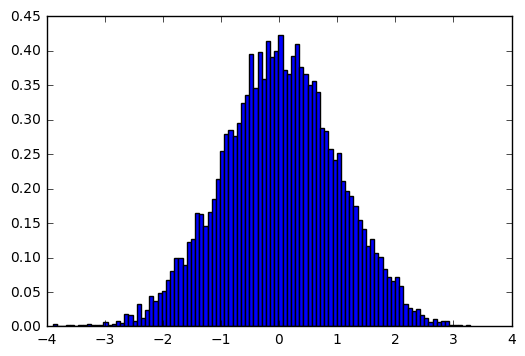
\includegraphics{output_196_0.png}
\caption{png}
\end{figure}

\begin{Shaded}
\begin{Highlighting}[]
\NormalTok{sigma }\OperatorTok{=} \DecValTok{1}\OperatorTok{;}\NormalTok{ mu }\OperatorTok{=} \DecValTok{0}
\end{Highlighting}
\end{Shaded}

\begin{Shaded}
\begin{Highlighting}[]
\NormalTok{norm_dist }\OperatorTok{=}\NormalTok{ (}\DecValTok{1}\OperatorTok{/}\NormalTok{np.sqrt(}\DecValTok{2}\OperatorTok{*}\NormalTok{sigma}\OperatorTok{*}\NormalTok{np.pi))}\OperatorTok{*}\NormalTok{np.exp(}\OperatorTok{-}\NormalTok{((bins}\OperatorTok{-}\NormalTok{mu)}\OperatorTok{**}\DecValTok{2}\NormalTok{)}\OperatorTok{/}\DecValTok{2}\NormalTok{)  }\CommentTok{#正态分布密度函数}
\end{Highlighting}
\end{Shaded}

\begin{Shaded}
\begin{Highlighting}[]
\NormalTok{matplotlib.pylab.plot(bins,norm_dist,color }\OperatorTok{=} \StringTok{'red'}\NormalTok{) }\CommentTok{#绘制正态分布密度函数图}
\end{Highlighting}
\end{Shaded}

\begin{verbatim}
[<matplotlib.lines.Line2D at 0x9308080>]
\end{verbatim}

\begin{figure}
\centering
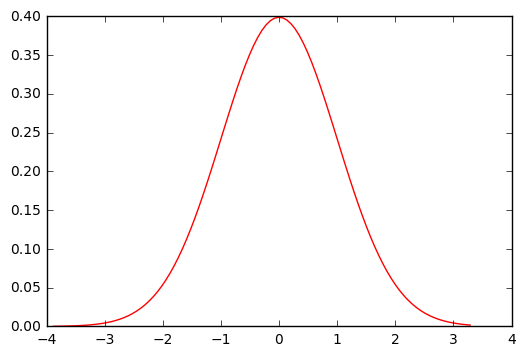
\includegraphics{output_199_1.png}
\caption{png}
\end{figure}

\subsubsection{使用二项分布进行赌博}

同时抛弃9枚硬币,如果正面朝上少于5枚,则输掉8元,否则就赢8元。如果手中有1000元作为赌资,请问赌博10000次后可能会是什么情况呢?

\begin{Shaded}
\begin{Highlighting}[]
\NormalTok{np.random.seed(}\DecValTok{1234}\NormalTok{)}
\end{Highlighting}
\end{Shaded}

\begin{Shaded}
\begin{Highlighting}[]
\NormalTok{binomial }\OperatorTok{=}\NormalTok{ np.random.binomial(}\DecValTok{9}\NormalTok{,}\FloatTok{0.5}\NormalTok{,}\DecValTok{10000}\NormalTok{) }\CommentTok{#生成二项分布随机数}
\end{Highlighting}
\end{Shaded}

\begin{Shaded}
\begin{Highlighting}[]
\NormalTok{money }\OperatorTok{=}\NormalTok{ np.zeros(}\DecValTok{10000}\NormalTok{) }\CommentTok{#生成10000次赌资的列表}
\end{Highlighting}
\end{Shaded}

\begin{Shaded}
\begin{Highlighting}[]
\NormalTok{money[}\DecValTok{0}\NormalTok{] }\OperatorTok{=} \DecValTok{1000} \CommentTok{#首次赌资为1000元}
\end{Highlighting}
\end{Shaded}

\begin{Shaded}
\begin{Highlighting}[]
\ControlFlowTok{for}\NormalTok{ i }\KeywordTok{in} \BuiltInTok{range}\NormalTok{(}\DecValTok{1}\NormalTok{,}\DecValTok{10000}\NormalTok{):}
    \ControlFlowTok{if}\NormalTok{ binomial[i] }\OperatorTok{<} \DecValTok{5}\NormalTok{:}
\NormalTok{        money[i] }\OperatorTok{=}\NormalTok{ money[i}\OperatorTok{-}\DecValTok{1}\NormalTok{] }\OperatorTok{-} \DecValTok{8}
    \ControlFlowTok{else}\NormalTok{:}
\NormalTok{        money[i] }\OperatorTok{=}\NormalTok{ money[i}\OperatorTok{-}\DecValTok{1}\NormalTok{] }\OperatorTok{+} \DecValTok{8}
\end{Highlighting}
\end{Shaded}

\begin{Shaded}
\begin{Highlighting}[]
\NormalTok{matplotlib.pylab.plot(np.arange(}\DecValTok{10000}\NormalTok{), money)}
\end{Highlighting}
\end{Shaded}

\begin{verbatim}
[<matplotlib.lines.Line2D at 0x964c588>]
\end{verbatim}

\begin{figure}
\centering
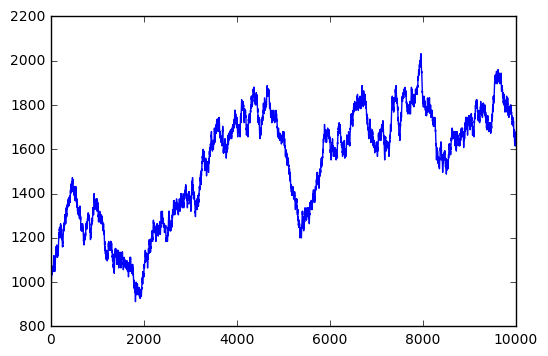
\includegraphics{output_207_1.png}
\caption{png}
\end{figure}

\subsubsection{使用随机整数实现随机游走}

一个醉汉在原始位置上行走10000步后将会在什么地方呢?如果他每走一步是随机的,即下一步可能是1也可能是-1。

\begin{Shaded}
\begin{Highlighting}[]
\NormalTok{np.random.seed(}\DecValTok{1234}\NormalTok{) }\CommentTok{#设定随机种子}
\end{Highlighting}
\end{Shaded}

\begin{Shaded}
\begin{Highlighting}[]
\NormalTok{position }\OperatorTok{=} \DecValTok{0} \CommentTok{#设置初始位置}
\end{Highlighting}
\end{Shaded}

\begin{Shaded}
\begin{Highlighting}[]
\NormalTok{walk }\OperatorTok{=}\NormalTok{ [] }\CommentTok{#创建空列表}
\end{Highlighting}
\end{Shaded}

\begin{Shaded}
\begin{Highlighting}[]
\NormalTok{steps }\OperatorTok{=} \DecValTok{10000} \CommentTok{#假设接下来行走10000步}
\end{Highlighting}
\end{Shaded}

\begin{Shaded}
\begin{Highlighting}[]
\ControlFlowTok{for}\NormalTok{ i }\KeywordTok{in}\NormalTok{ np.arange(steps):}
\NormalTok{    step }\OperatorTok{=} \DecValTok{1} \ControlFlowTok{if}\NormalTok{ np.random.randint(}\DecValTok{0}\NormalTok{,}\DecValTok{2}\NormalTok{) }\ControlFlowTok{else} \OperatorTok{-}\DecValTok{1} \CommentTok{#每一步都是随机的}
\NormalTok{    position }\OperatorTok{=}\NormalTok{ position }\OperatorTok{+}\NormalTok{ step }\CommentTok{#对每一步进行累计求和}
\NormalTok{    walk.append(position) }\CommentTok{#确定每一步所在的位置}
\end{Highlighting}
\end{Shaded}

\begin{Shaded}
\begin{Highlighting}[]
\NormalTok{matplotlib.pylab.plot(np.arange(}\DecValTok{10000}\NormalTok{),walk) }\CommentTok{#绘制随机游走图}
\end{Highlighting}
\end{Shaded}

\begin{verbatim}
[<matplotlib.lines.Line2D at 0xa088860>]
\end{verbatim}

\begin{figure}
\centering
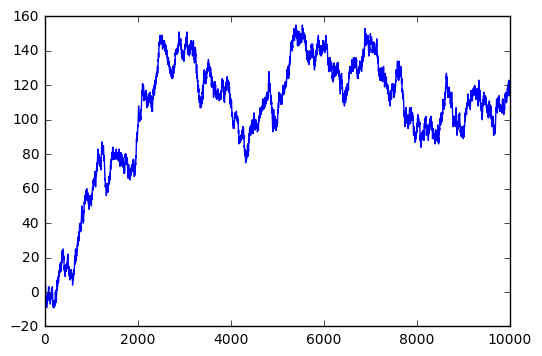
\includegraphics{output_215_1.png}
\caption{png}
\end{figure}

上面的代码还可以写成(结合前面所讲的where函数,cumsum函数):

\begin{Shaded}
\begin{Highlighting}[]
\NormalTok{np.random.seed(}\DecValTok{1234}\NormalTok{)}
\end{Highlighting}
\end{Shaded}

\begin{Shaded}
\begin{Highlighting}[]
\NormalTok{step }\OperatorTok{=}\NormalTok{ np.where(np.random.randint(}\DecValTok{0}\NormalTok{,}\DecValTok{2}\NormalTok{,}\DecValTok{10000}\NormalTok{) }\OperatorTok{>} \DecValTok{0}\NormalTok{,}\DecValTok{1}\NormalTok{,}\OperatorTok{-}\DecValTok{1}\NormalTok{)}
\end{Highlighting}
\end{Shaded}

\begin{Shaded}
\begin{Highlighting}[]
\NormalTok{position }\OperatorTok{=}\NormalTok{ np.cumsum(step)}
\end{Highlighting}
\end{Shaded}

\begin{Shaded}
\begin{Highlighting}[]
\NormalTok{matplotlib.pylab.plot(np.arange(}\DecValTok{10000}\NormalTok{), position)}
\end{Highlighting}
\end{Shaded}

\begin{verbatim}
[<matplotlib.lines.Line2D at 0xa5e5908>]
\end{verbatim}

\begin{figure}
\centering
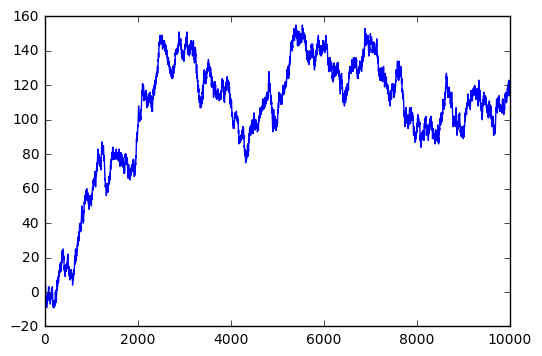
\includegraphics{output_220_1.png}
\caption{png}
\end{figure}

避免for循环,可以达到同样的效果。

以上就是numpy的基本内容。


\end{document}
